\documentclass{beamer}

\usepackage[T2A]{fontenc}
\usepackage[utf8x]{inputenc}
\usepackage[english,bulgarian]{babel}
\usepackage{multirow}

\mode<presentation> {
	\usetheme{Berlin}
}

%\usebackgroundtemplate {
%	\includegraphics[width=370px, height=270px, trim=0 0 0 -80px]{background}
%}

\graphicspath{{../images/}}

\title{Инсталация и стартиране}
\subtitle{Статистическа обработка на данни с R}

\author{Пламен Петров и Тодор Балабанов}

\date{30.IV.2020}

\institute[ЦО и ИИКТ към БАН] {
	Център за обучение \\
	Институт по информационни и комуникационни технологии \\ 
	Българската академия на науките \\
	\medskip
	\textit{p.petrov@iit.bas.bg todorb@iinf.bas.bg}
}

\addtobeamertemplate{navigation symbols}{}{
	\usebeamerfont{footline}
	\usebeamercolor[fg]{footline}
	\hspace{1em}
	\insertframenumber/\inserttotalframenumber
}

\begin{document}

\begin{frame}
	\titlepage
\end{frame}

\section*{Теми}
\begin{frame}[shrink]
	\frametitle{Съдържание}
	\tableofcontents
\end{frame}

\section{Изтегляне на инсталационните файлове}

\begin{frame}
\center \huge{Изтегляне на инсталационните файлове}
\end{frame}

\subsection{Източник с инсталационни файлове}

\begin{frame}
\frametitle{Начална уеб страница на продукта}
\begin{figure}[]
\includegraphics[width=\textwidth,height=0.75\textheight]{pic0001}\end{figure}
\end{frame}

\begin{frame}
\frametitle{Списък със сървъри за изтегляне}
\begin{figure}[]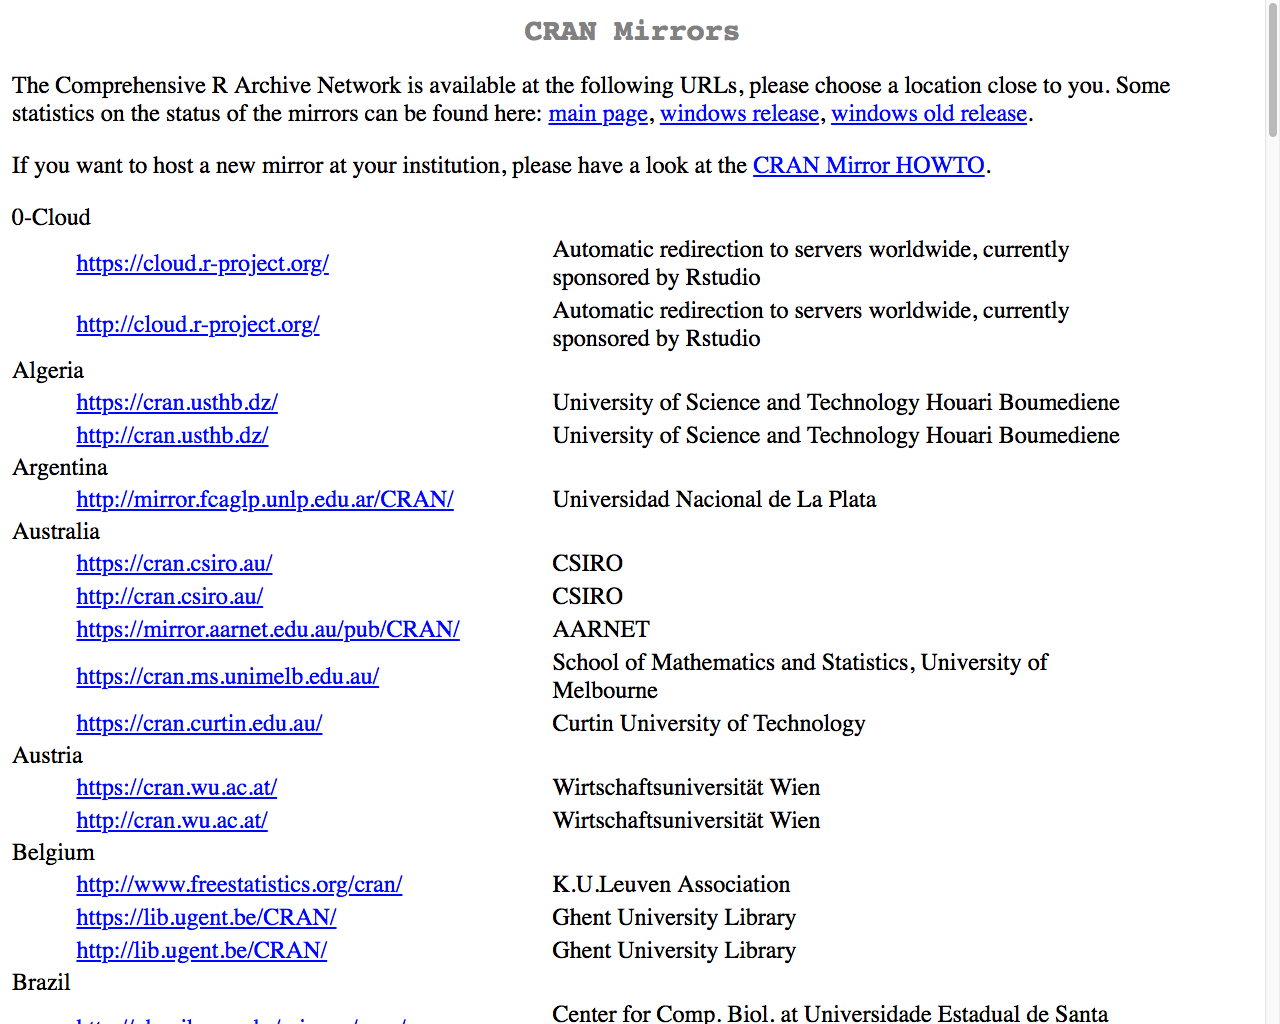
\includegraphics[width=\textwidth,height=0.75\textheight]{pic0002}\end{figure}
\end{frame}

\subsection{Избор на инсталационен файл и версия}

\begin{frame}
\frametitle{Избор на подходяща инсталация за операционната система}
\begin{figure}[]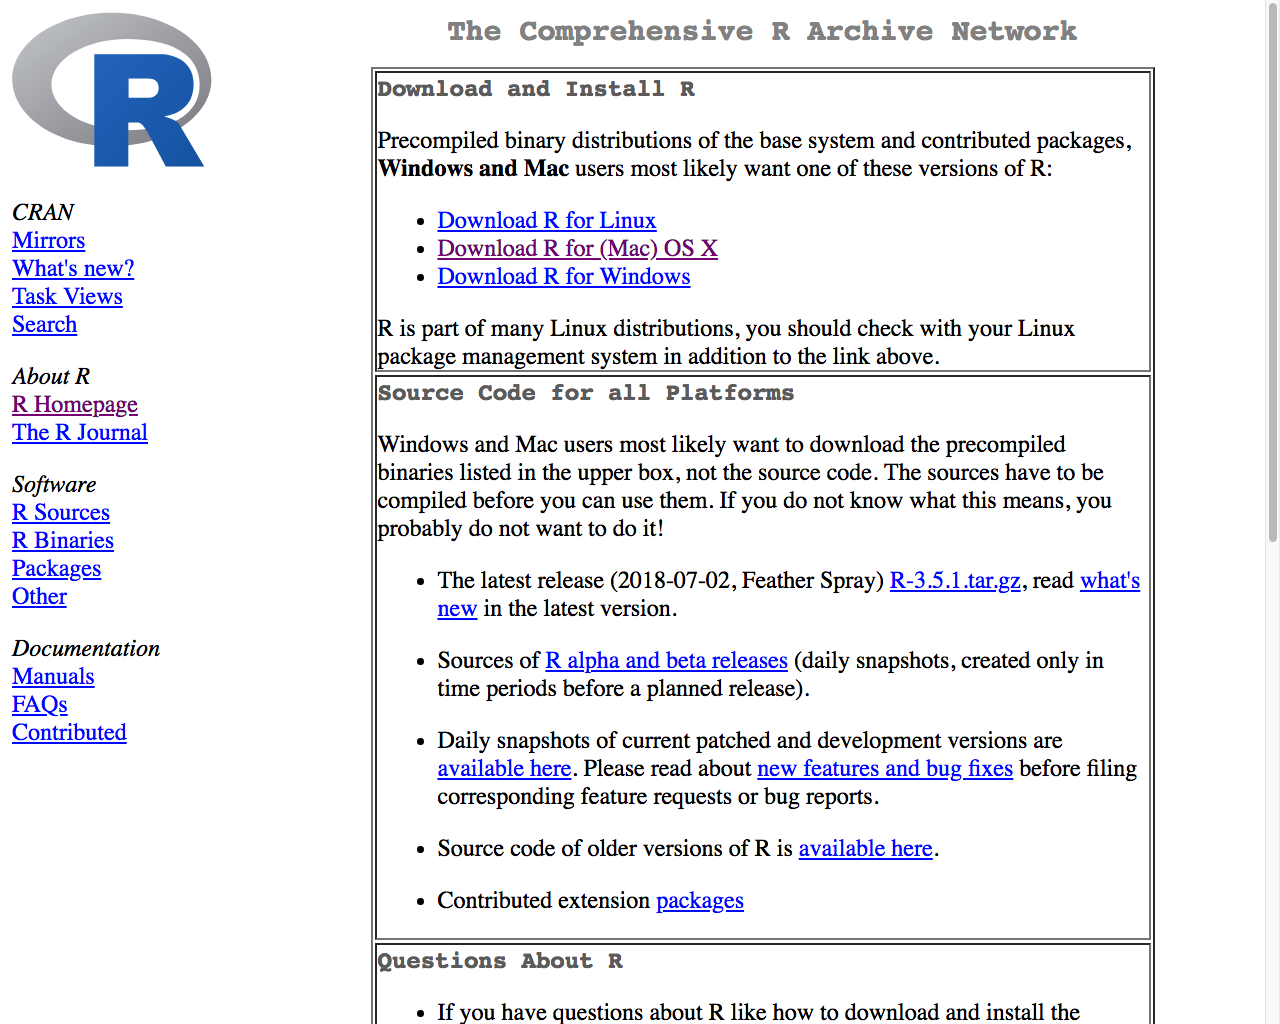
\includegraphics[width=\textwidth,height=0.75\textheight]{pic0003}\end{figure}
\end{frame}

\begin{frame}
\frametitle{Избор на версия за изтегляне}
\begin{figure}[]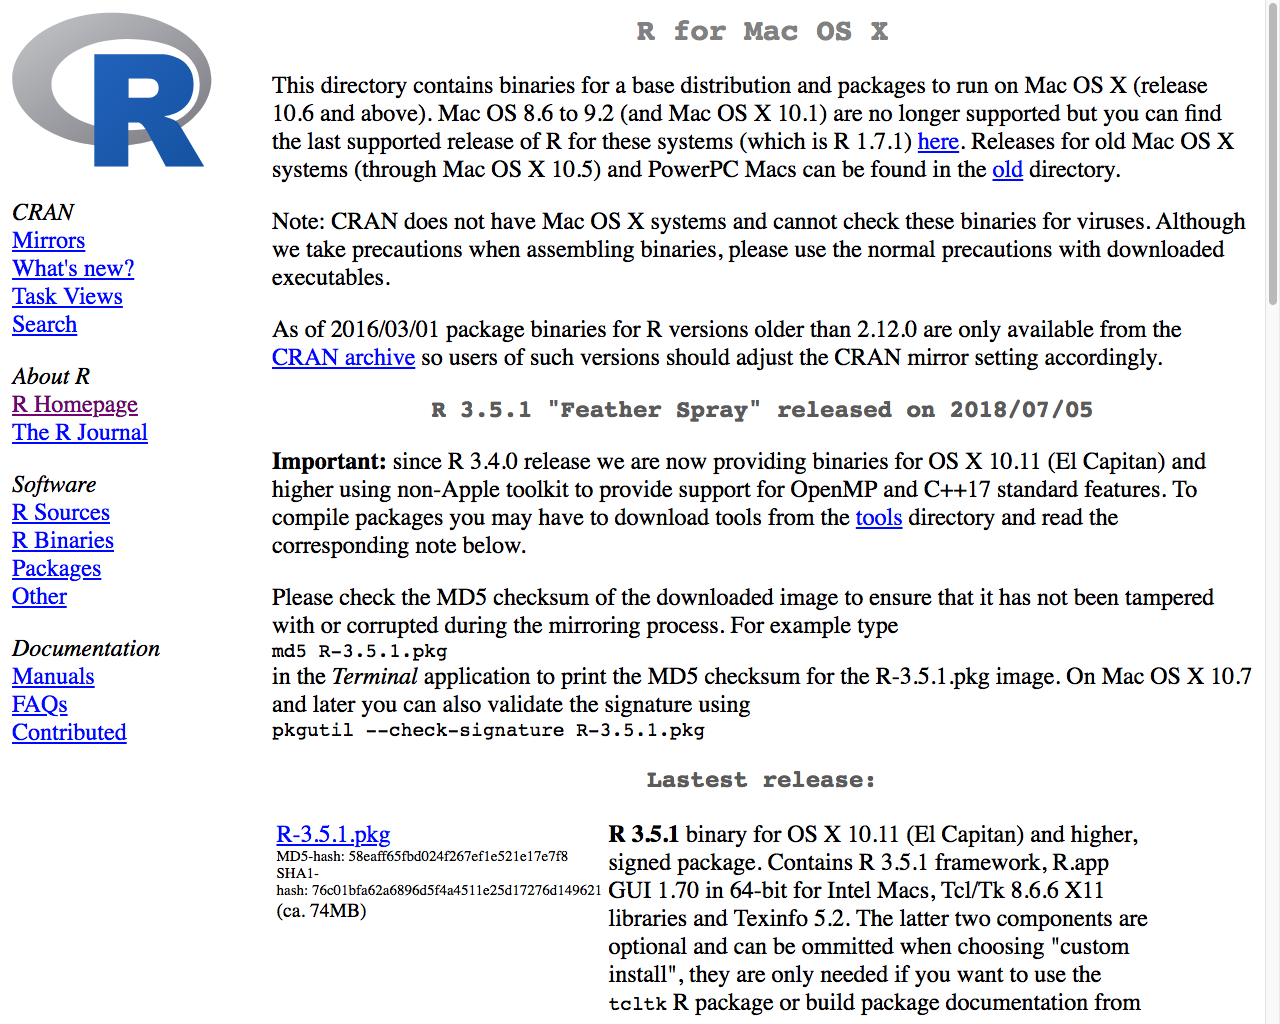
\includegraphics[width=\textwidth,height=0.75\textheight]{pic0004}\end{figure}
\end{frame}

\begin{frame}
\frametitle{Запазване на инсталационния файл}
\begin{figure}[]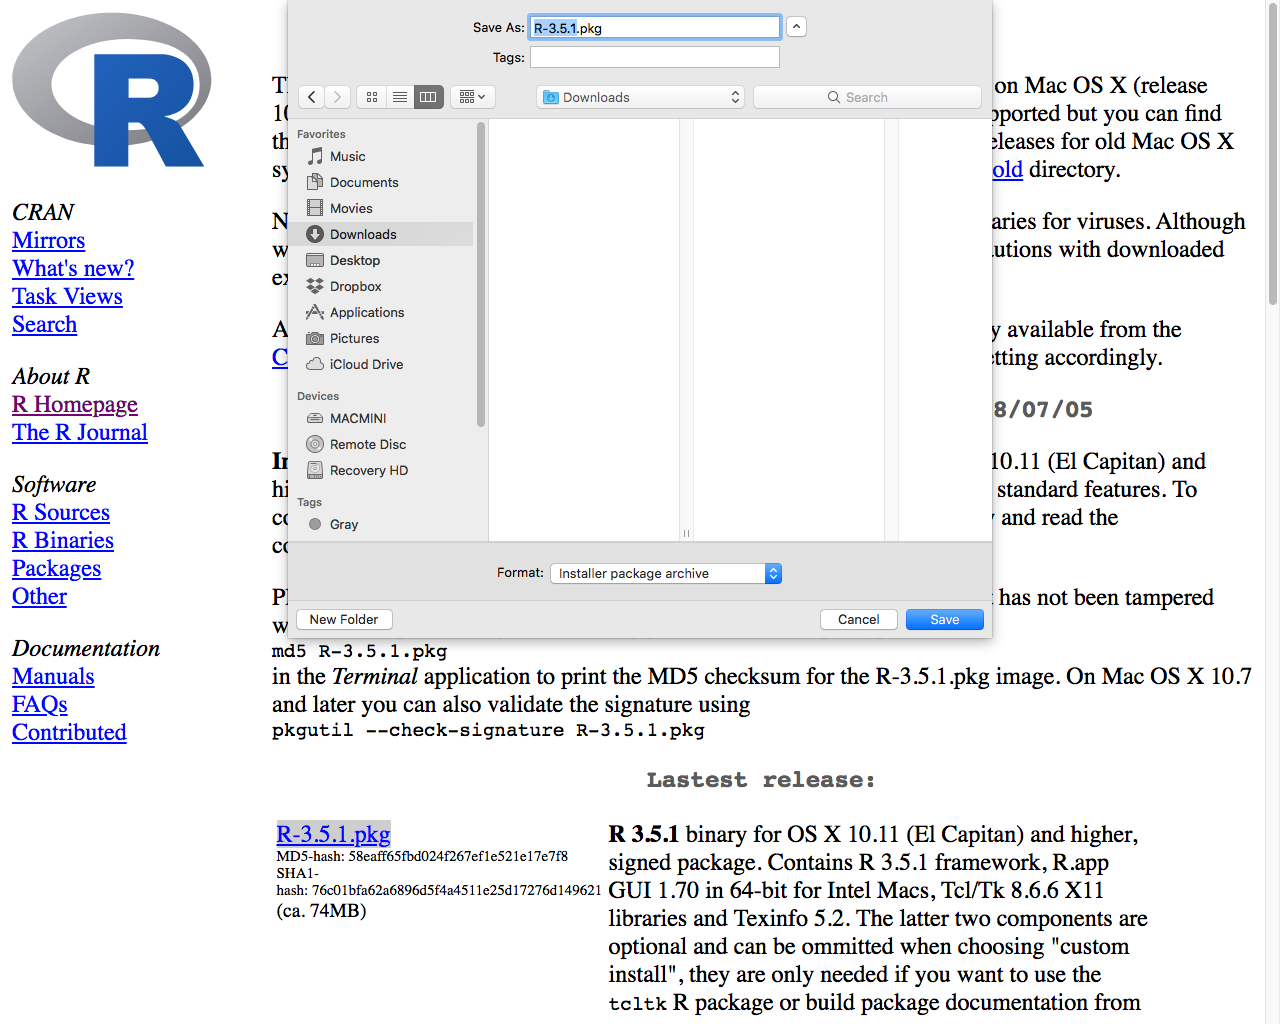
\includegraphics[width=\textwidth,height=0.75\textheight]{pic0005}\end{figure}
\end{frame}

\section{Инсталация}

\begin{frame}
\center \huge{Инсталация}
\end{frame}

\subsection{Инсталатор}

\begin{frame}
\frametitle{Активиране на инсталатора}
\begin{figure}[]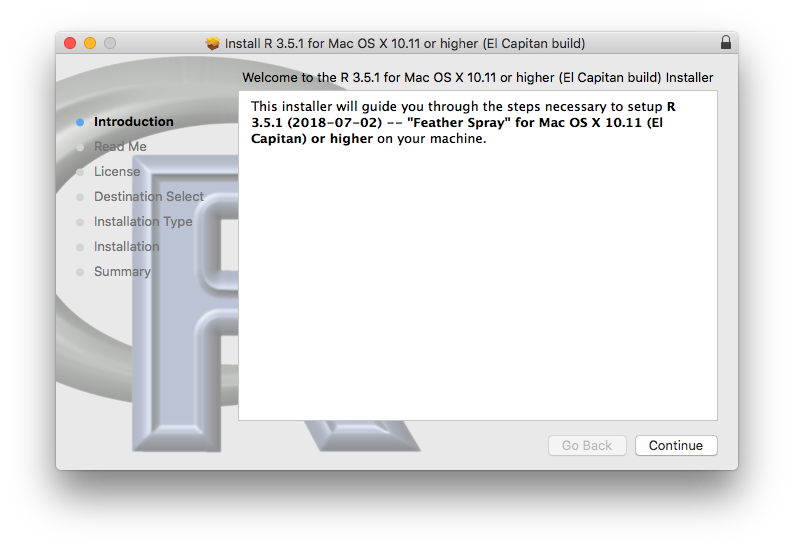
\includegraphics[width=\textwidth,height=0.75\textheight]{pic0006}\end{figure}
\end{frame}

\begin{frame}
\frametitle{Подробности за инсталацията}
\begin{figure}[]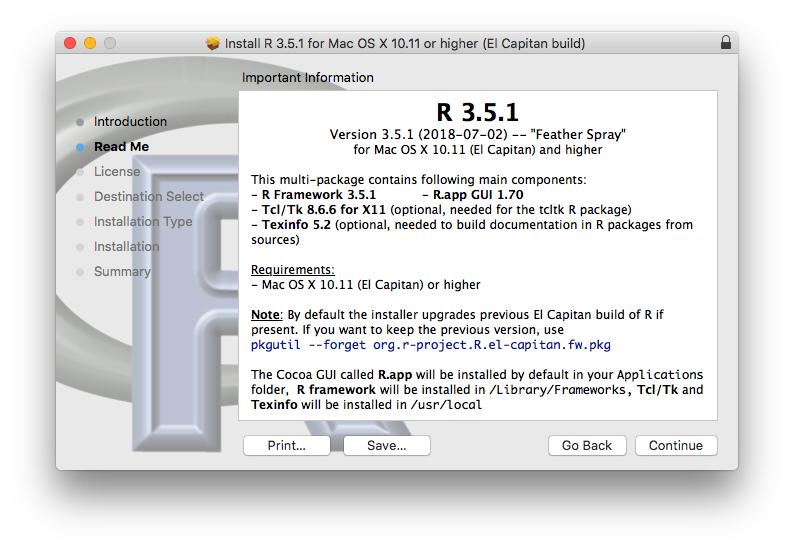
\includegraphics[width=\textwidth,height=0.75\textheight]{pic0007}\end{figure}
\end{frame}

\subsection{Съгласие от потребителя}

\begin{frame}
\frametitle{Лицензно споразумение за ползване}
\begin{figure}[]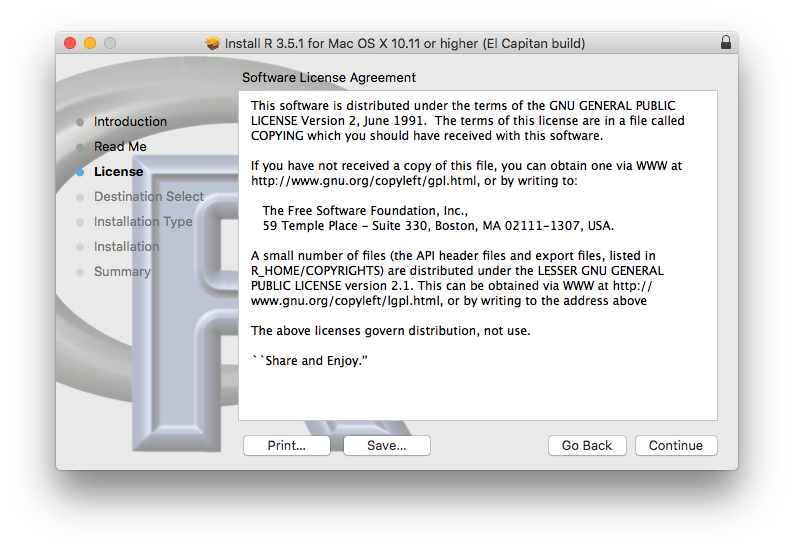
\includegraphics[width=\textwidth,height=0.75\textheight]{pic0008}\end{figure}
\end{frame}

\begin{frame}
\frametitle{Изрично съгласие}
\begin{figure}[]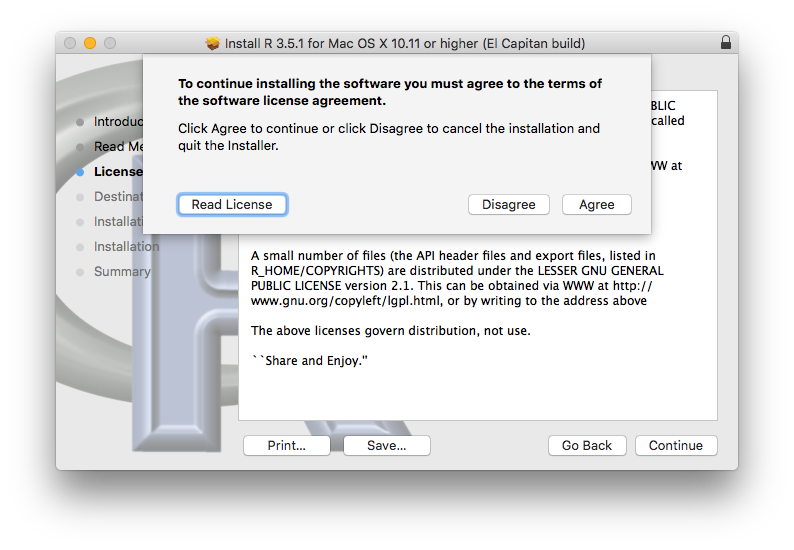
\includegraphics[width=\textwidth,height=0.75\textheight]{pic0009}\end{figure}
\end{frame}

\subsection{Резултат от инсталацията}

\begin{frame}
\frametitle{Информация за директорията и използваното дисково пространство}
\begin{figure}[]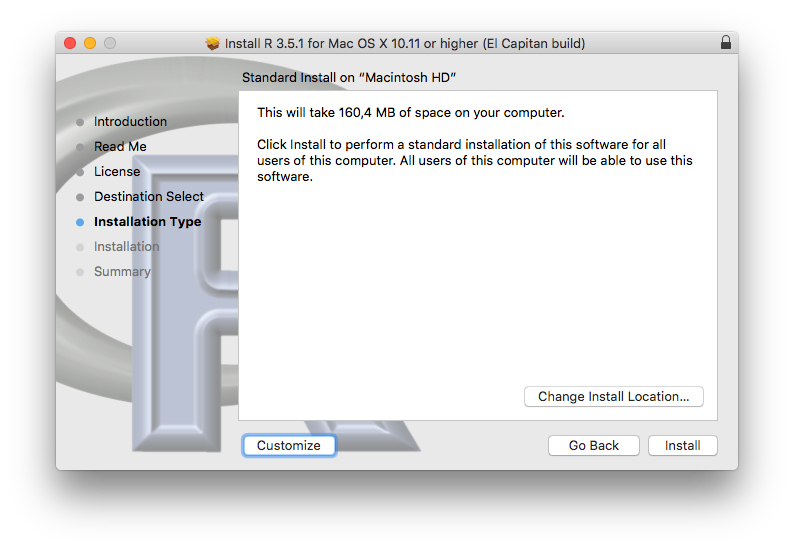
\includegraphics[width=\textwidth,height=0.75\textheight]{pic0010}\end{figure}
\end{frame}

\begin{frame}
\frametitle{Успешно приключване на инсталацията}
\begin{figure}[]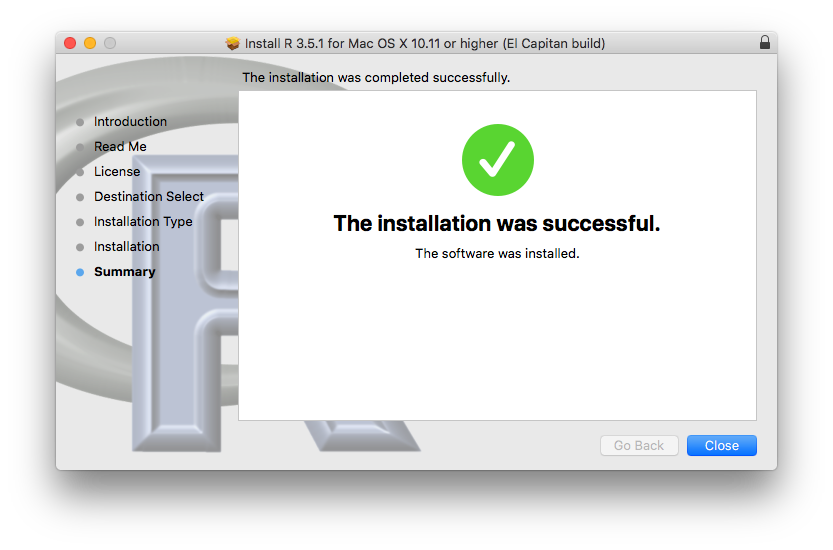
\includegraphics[width=\textwidth,height=0.75\textheight]{pic0011}\end{figure}
\end{frame}

\section{Работа в режим на команди}

\begin{frame}
\center \huge{Работа в режим на команди}
\end{frame}

\subsection{Изглед и команди}

\begin{frame}
\frametitle{Основен прозорец на продукта}
\begin{figure}[]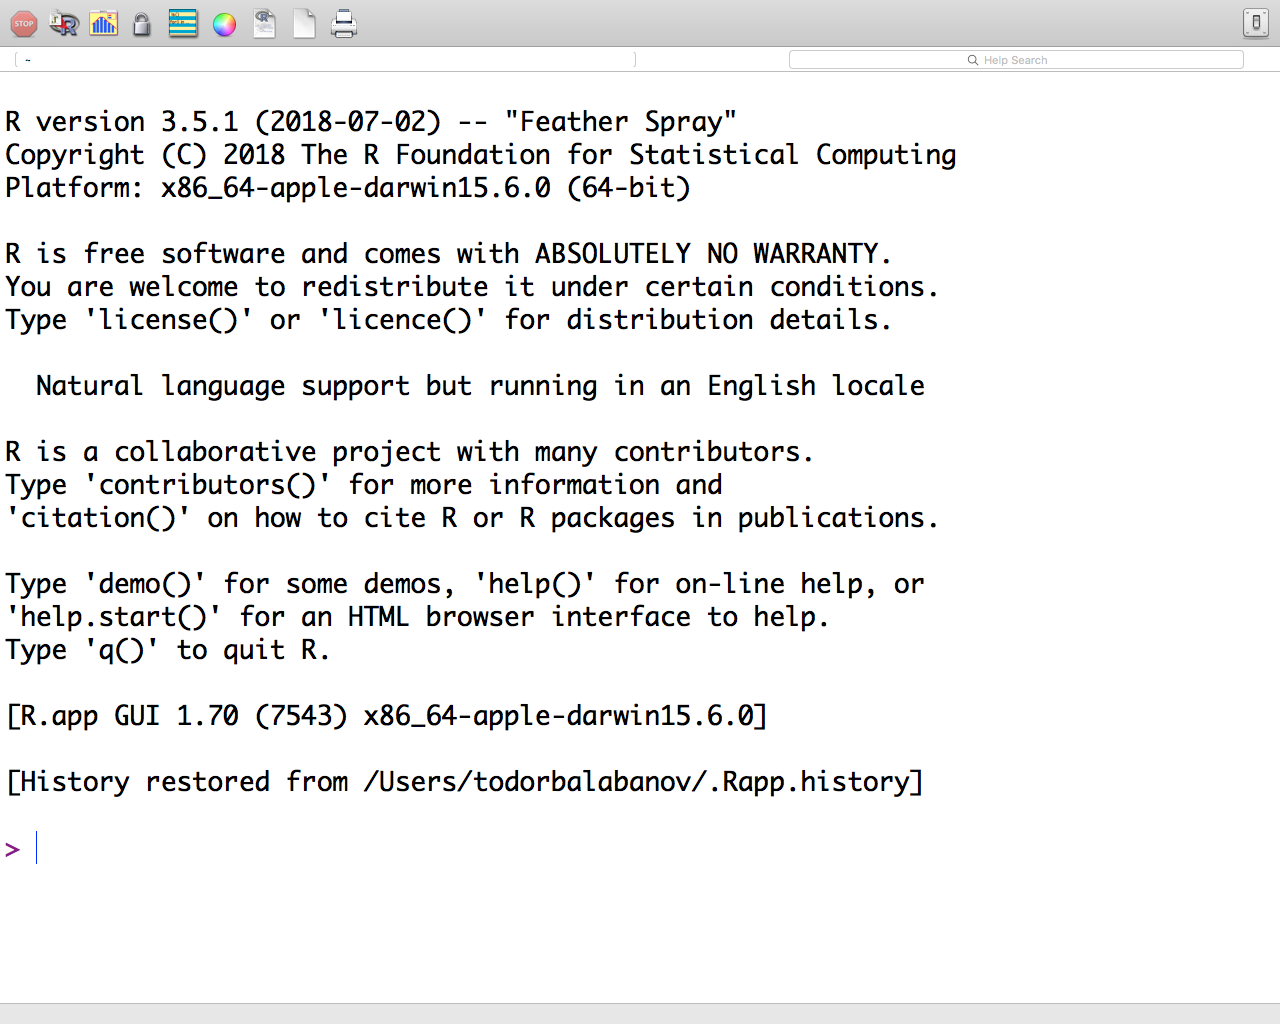
\includegraphics[width=\textwidth,height=0.75\textheight]{pic0012}\end{figure}
\end{frame}

\begin{frame}
\frametitle{Изпълнение на команда за печат}
\begin{figure}[]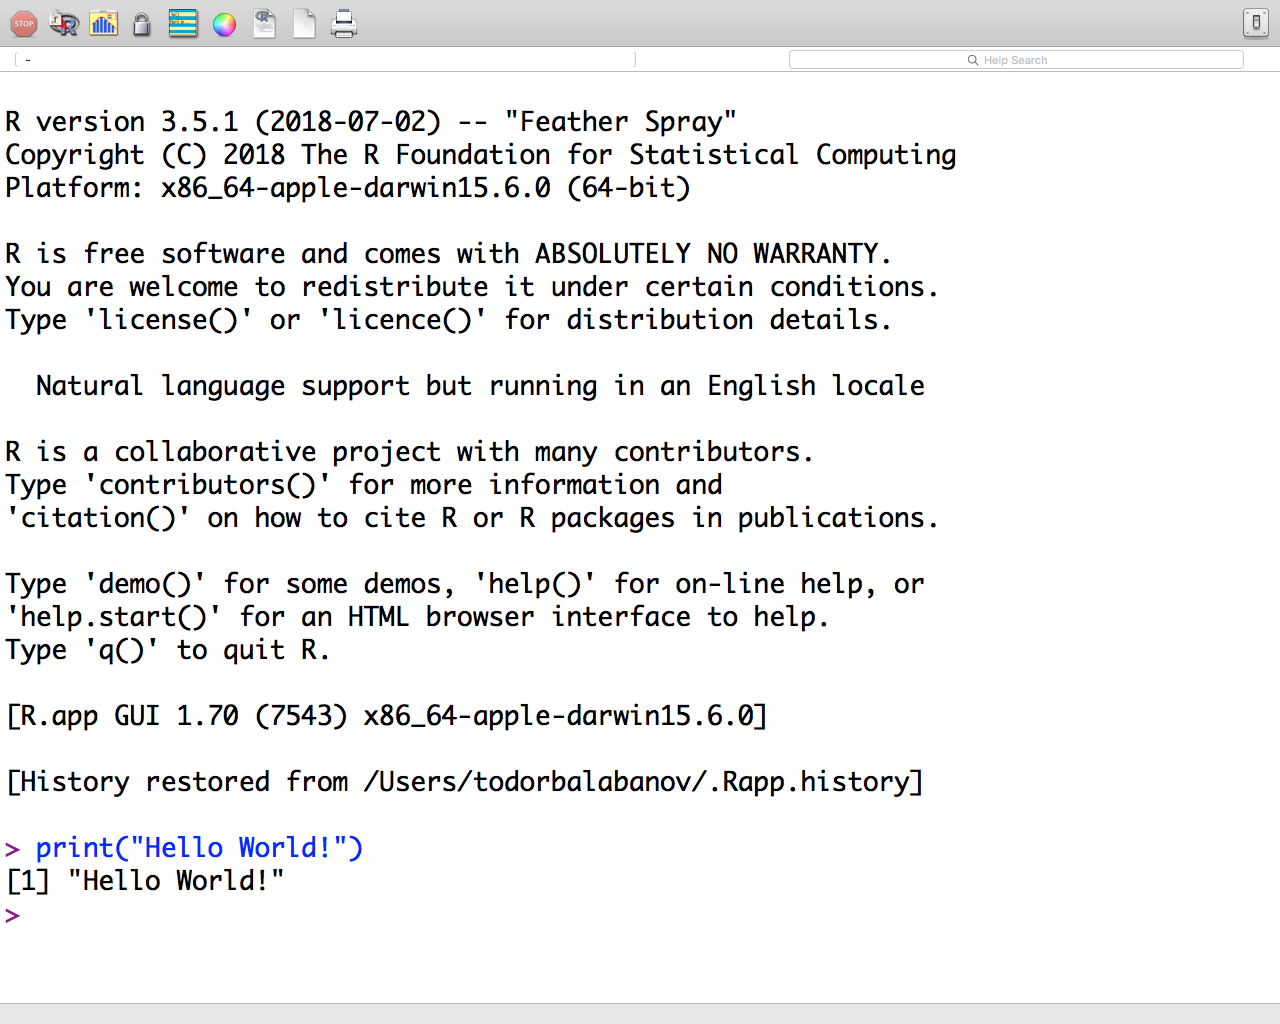
\includegraphics[width=\textwidth,height=0.75\textheight]{pic0013}\end{figure}
\end{frame}

\section{Заключение}

\begin{frame}
\center \huge{Заключение}
\end{frame}

\subsection{Дискусия}

\begin{frame}
\frametitle{Въпроси и отговори}
\center \huge{Благодаря за вниманието!}
\end{frame}

\end{document}
